\chapter{Streaming Readout}
\label{chap:streaming_readout}

As proposed in Chapter~\ref{chap:beam_use_proposal}, the sPHENIX data taking will start with Au+Au collisions in 2023, followed by XXXX-week of \pp and YYYY-week of p+A collisions in 2024.  In the first three years of sPHENIX operation, the collaboration envisions a run plan sampling 2 trillion \pp collisions (50~$pb^{-1}$)  with electron and jet triggers, as well as recording 140 billion M.B. Au+Au collisions. Comparison of the A+A HF observables to that of the \pp data reveals how the HF probes interact with QGP. However, due to the rareness of the HF signals in the \pp collisions, the currently envisioned sPHENIX detector equipped with a traditional triggered  DAQ cannot efficiently sample HF production below a $p_T$ of 10 GeV$/c$. 
 
A study~[SRO tech note] found that the sPHENIX tracking detectors can be upgraded to record a large amount of \pp collisions via a streaming readout upgrade in the data acquisition (DAQ) firmware and software. 
(Embed something we want PAC to write in report) 
This chapter will discuss the proposed implementation and benefit of this upgrade. 
 

 
\section{Streaming Readout Upgrade}
 
 The currently envisioned sPHENIX experiment is designed to take large statistics of calorimeter triggered events in the \pp collisions, which will sample 2 trillion delivered \pp collisions in the vertex acceptance of the silicon tracker (18\% of all collisions) []. For observables that utilize calorimeter for analysis, a trigger can usually be designed, such as leptonic decays at higher $p_T$, jets, photon, and their correlation observables. However, low-$p_T$  ($<10$ GeV$/c$) HF hadrons usually decay hadronically and leave relatively low signals in the calorimeters when compared with the underlying event. Therefore, they cannot be efficiently collected via calorimeter triggers, which have a hadron energy threshold of 10 GeV. Therefore, in the currently envisioned sPHENIX detector, there is no efficient way in triggering such events in the \pp collisions. And in the 15 kHz sPHENIX trigger bandwidth, one would only reasonable request around few kHz of the minimum bias \pp trigger for this new program. Assuming 50\% vertex range selection purity , 1 kHz M.B. trigger leads to recording $2\times10^{-4}$ of the delivered luminosity . This translates to quite limited statistics for these rare low-$p_T$ HF signals as quantified in Table X.
 
 The upgraded DAQ is illustrated in Figure X and summarized in Table X. For all three tracking detectors, their FEE and DAQ hardware supports the streaming mode and provides the capability needed for this upgrade. The main work will focus on DAQ firmware and software development that enabling the streaming capability. 
This upgrade carries out the upgrade enabling the collection of a sufficient amount of minimum bias \pp events. That is 10\% delivered luminosity (see next Chapter), 200 billion events in vertex tracker acceptance, which is a factor of 500 improvements. This dataset enables a comprehensive low-$p_T$ hadron program as discussed in this subsection. The analysis for these HF hadronic channels does not require calorimeter information. Instead, as illustrated in Figure X, they can be identified with the precision tracking detectors of sPHENIX (at $p_T$=5 GeV$/c$, $\sigma(p)/p=1\%$, $\sigma(DCA)<10$~$\mu$m ) via a combination of decay topology and invariant mass, as demonstrated for even the busiest events of Au+Au collisions through detailed simulation studies in []. 
 
(Year 4-5 agressive SRO)

\section{Physics Benefit of Streaming Readout Upgrade in Run24}
 
 As summarized in Table ??, upgraded DAQ for sPHENIX trackers will stream recording 500 times higher statistics of M.B. \pp collisions, which will enable the HF measurements in this key kinematic region.


\section{\pp~baseline for bottom $R_{AA}$}


\begin{figure}[htbp]
\begin{center}
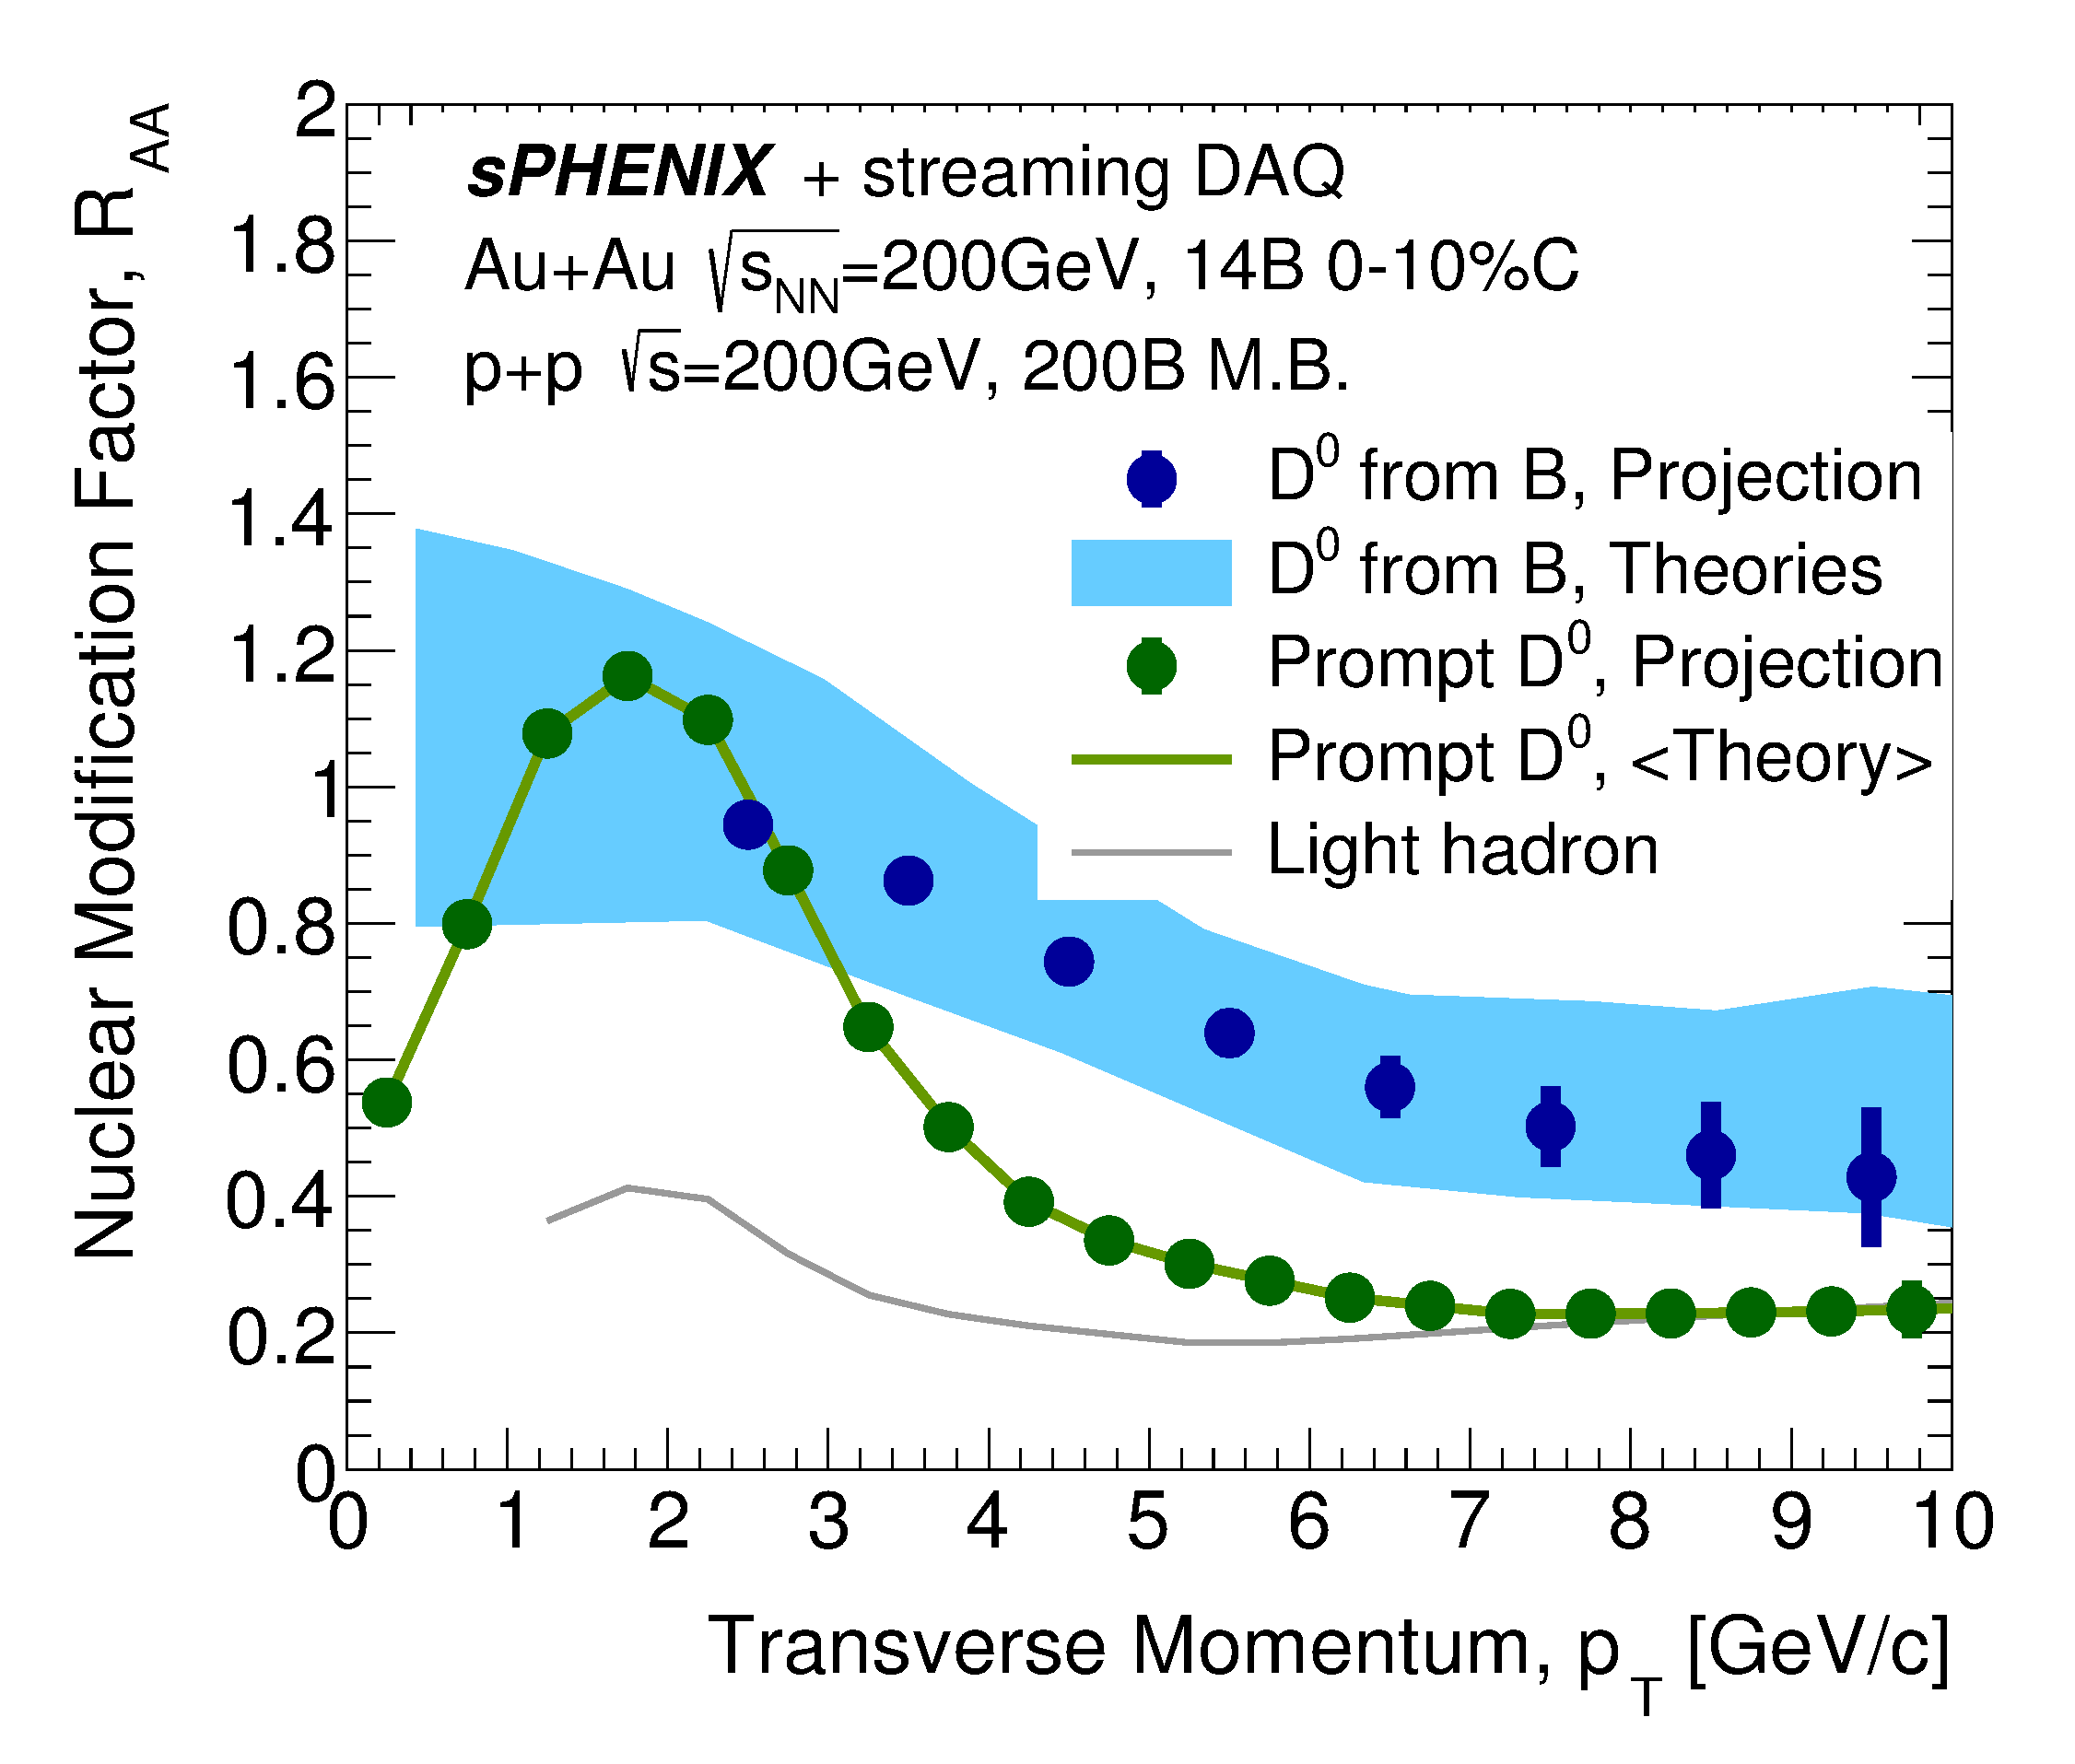
\includegraphics[width=.49\linewidth]{figs/RAA_DB_theory_root_RAADB_pp200B.pdf}
% 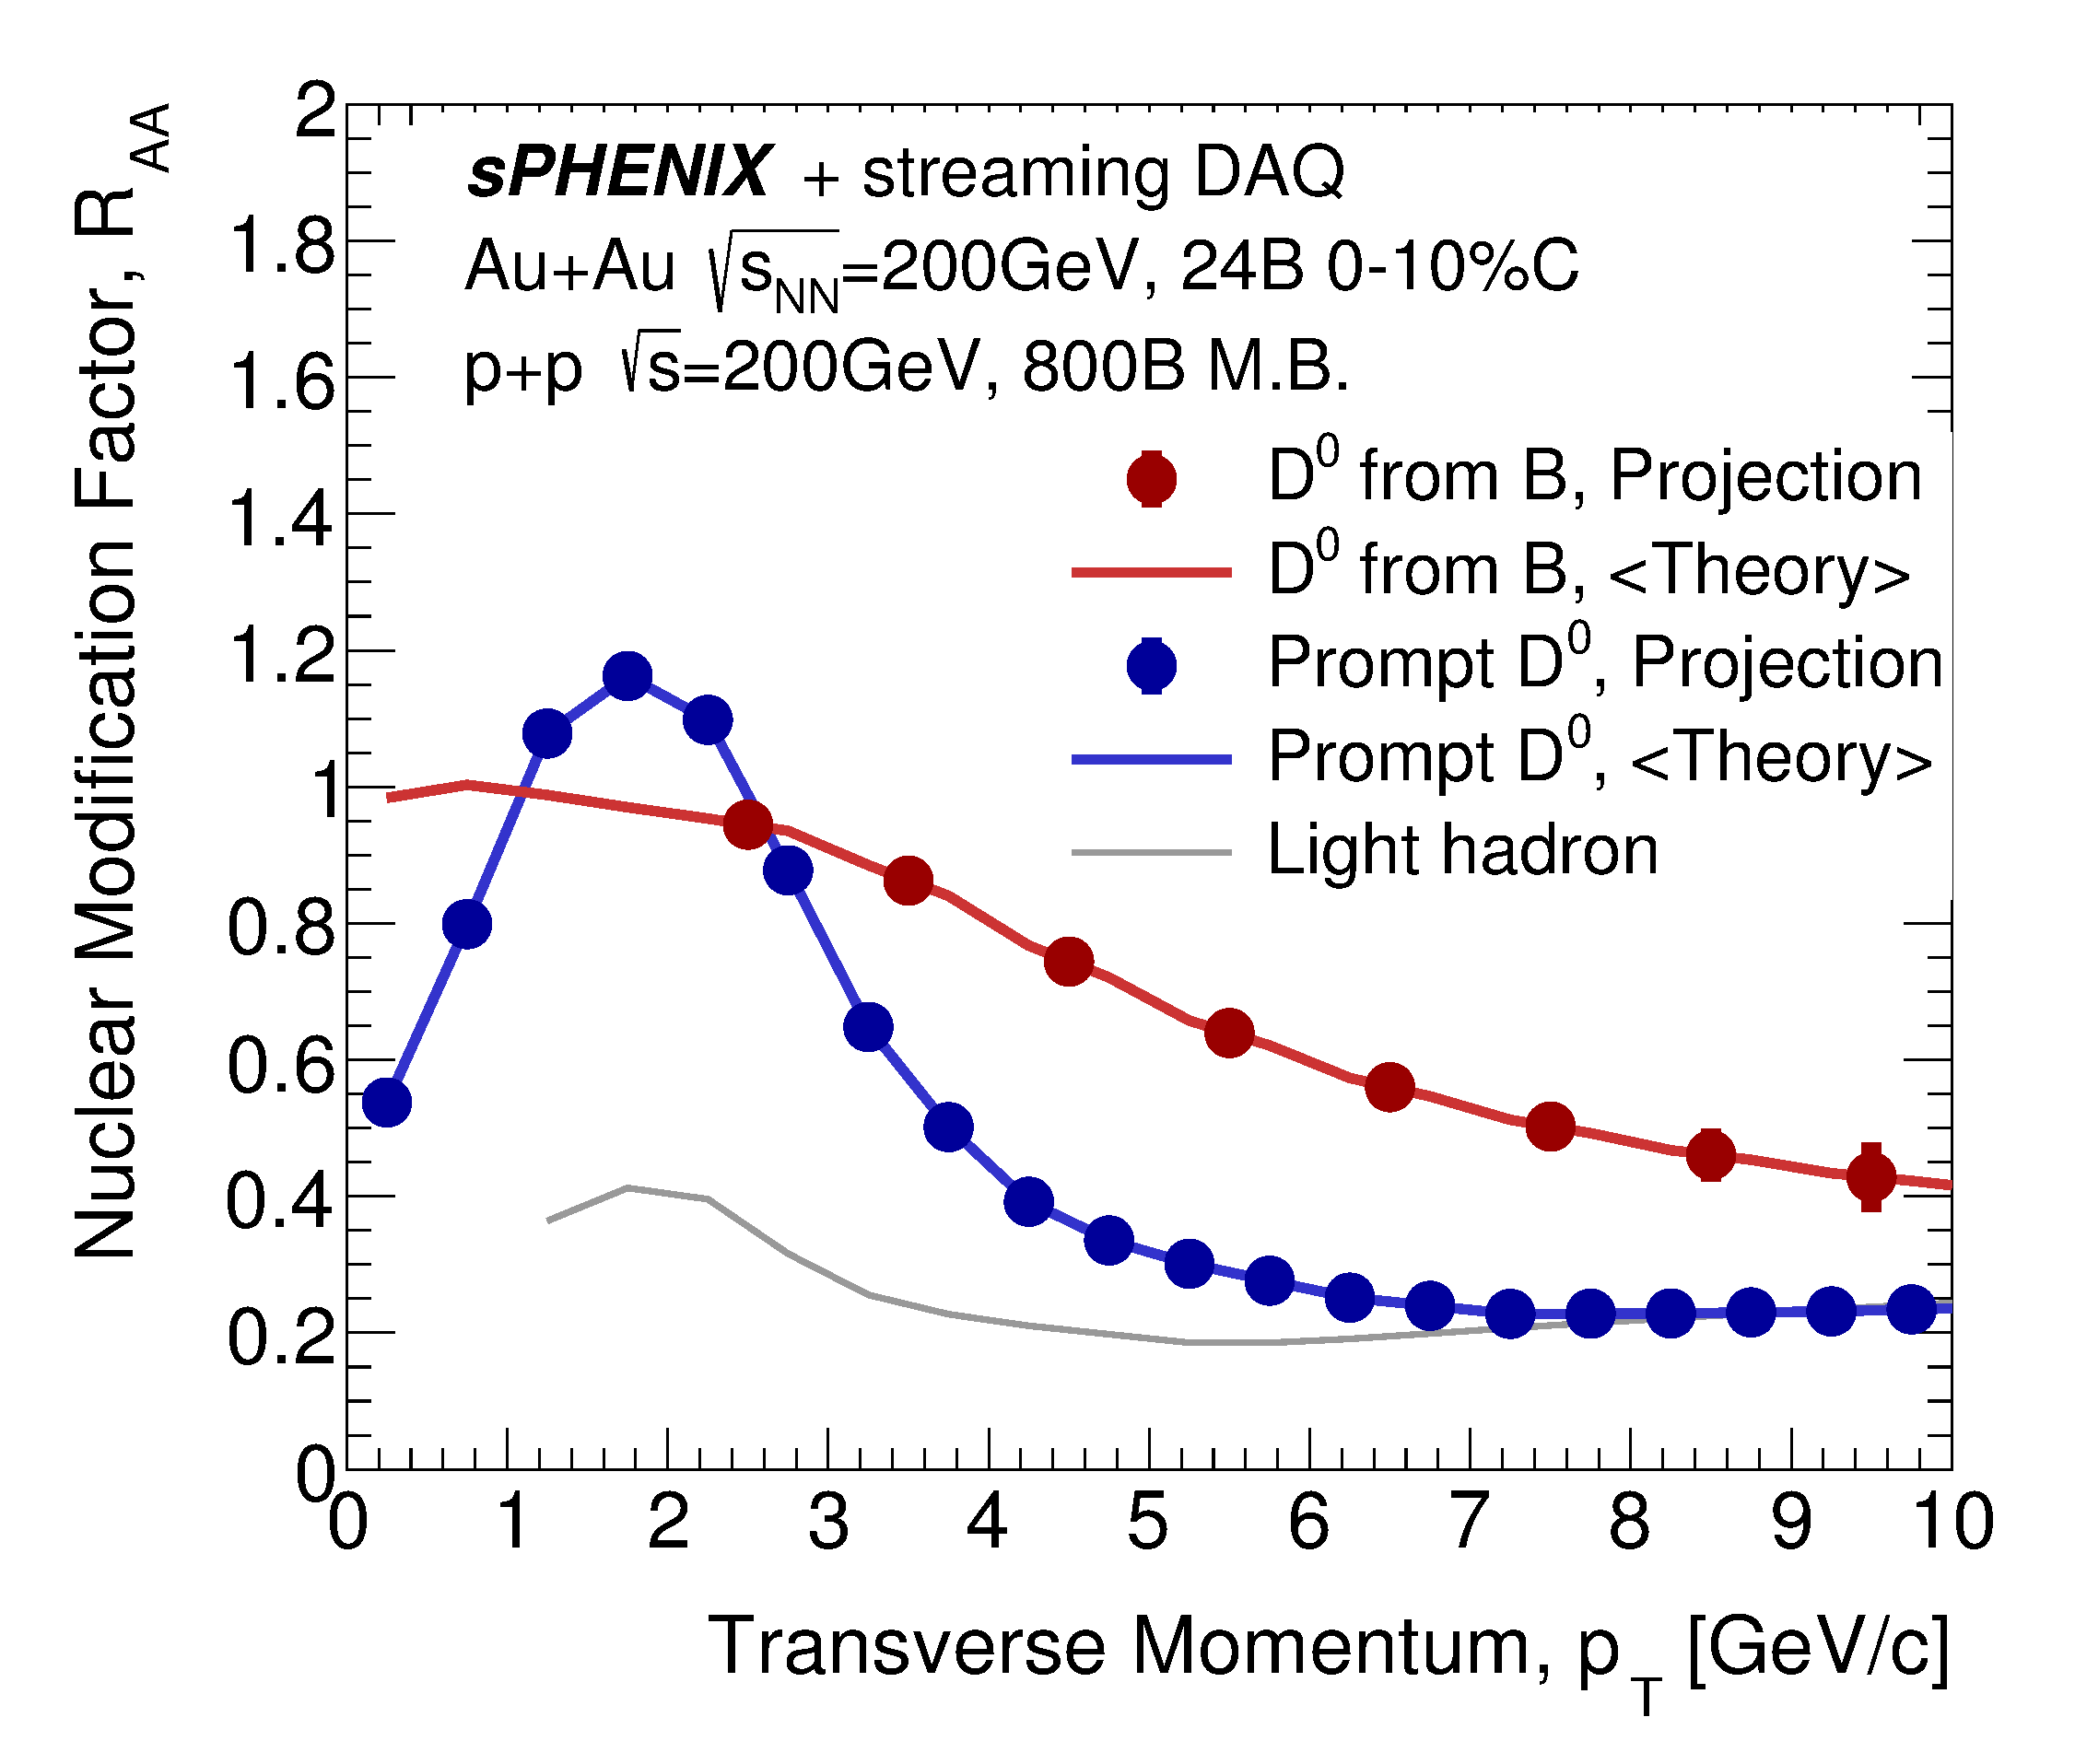
\includegraphics[width=.49\linewidth]{figs/RAA_DB_theory_root_RAADB.pdf}
\caption{Statistical projections of $R_AA$ for $D^0$ from $B$ decays for Year-2 data taking.}
\label{fig:RAA-D0}
\end{center}
\end{figure}



The currently envisioned sPHENIX experiment is designed to take large statistics of calorimeter triggered events in the \pp collisions, which will sample 2 trillion delivered \pp collisions in the vertex acceptance of the silicon tracker (18\% of all collisions) []. For observables that utilize calorimeter for analysis, a trigger can usually be designed, such as leptonic decays at higher $p_T$, jets, photon, and their correlation observables. However, low-$p_T$  ($<10$~GeV$/c$) HF hadrons usually decay hadronically and leave relatively low signals in the calorimeters when compared with the underlying event. Therefore, they cannot be efficiently collected via calorimeter triggers, which have a hadron energy threshold of 10 GeV. Therefore, in the currently envisioned sPHENIX detector, there is no efficient way in triggering such events in the \pp collisions. And in the 15 kHz sPHENIX trigger bandwidth, one would only reasonable request around few kHz of the minimum bias \pp trigger for this new program. Assuming 50\% vertex range selection purity , 1 kHz M.B. trigger leads to recording $2\times10^{-4}$ of the delivered luminosity . This translates to quite limited statistics for these rare low-$p_T$ HF signals as quantified in Table X [Need table].
This upgrade carries out the upgrade enabling the collection of a sufficient amount of minimum bias \pp events. That is 10\% delivered luminosity (see next Chapter), 200 billion events in vertex tracker acceptance, which is a factor of 500 improvements. This dataset enables a comprehensive low-$p_T$ hadron program as discussed in this subsection. The analysis for these HF hadronic channels does not require calorimeter information. Instead, they can be identified with the precision tracking detectors of sPHENIX (at $p_T$=5 GeV$/c$, $\sigma(p)/p=1\%$, $\sigma(DCA)<10$~$\mu$m ) via a combination of decay topology and invariant mass, as demonstrated for even the busiest events of Au+Au collisions through detailed simulation studies in [?]. 
 
 
The non-prompt $D^0$ meson production is a clean channel to access b-quark via its decay chain. Using tracker data alone, both prompt and non-prompt $D^0$ can be reconstructed via the invariant mass and a multi-variable classification algorithm based on the decay topology, including the distance of closest approach ($DCA$) of tracks, the closeness between tracks, decay length and angle, as demonstrated in a worse background situation (A+A) in []. Together with the sPHENIX Au+Au dataset, this upgrade will enable the first precision measurement of nuclear modification of the B observable at RHIC via the non-prompt $D^0$ as highlighted in Figure~\ref{fig:RAA-D0}. Similar measurement will be expanded to the exclusive decay modes such as $B^+ \rightarrow \pi^+ (D^0 \rightarrow \pi^- K^+)$) (~1k events expected).

With the extensive, inclusive dataset, the SRO upgrade will further enable novel highly differential observables, such as the $c$-quark correlation measurement by detecting pairs of $D^0$ mesons. 500k $D^0$ pairs will be recorded with the upgraded DAQ. Together with the planned Au+Au data, such dataset for Charm correlations will provide a unique handle in quantitatively understanding the diffusion of c-quarks in QGP []. 

\section{Charm Hadronization}


\begin{figure}[htbp]
\begin{center}
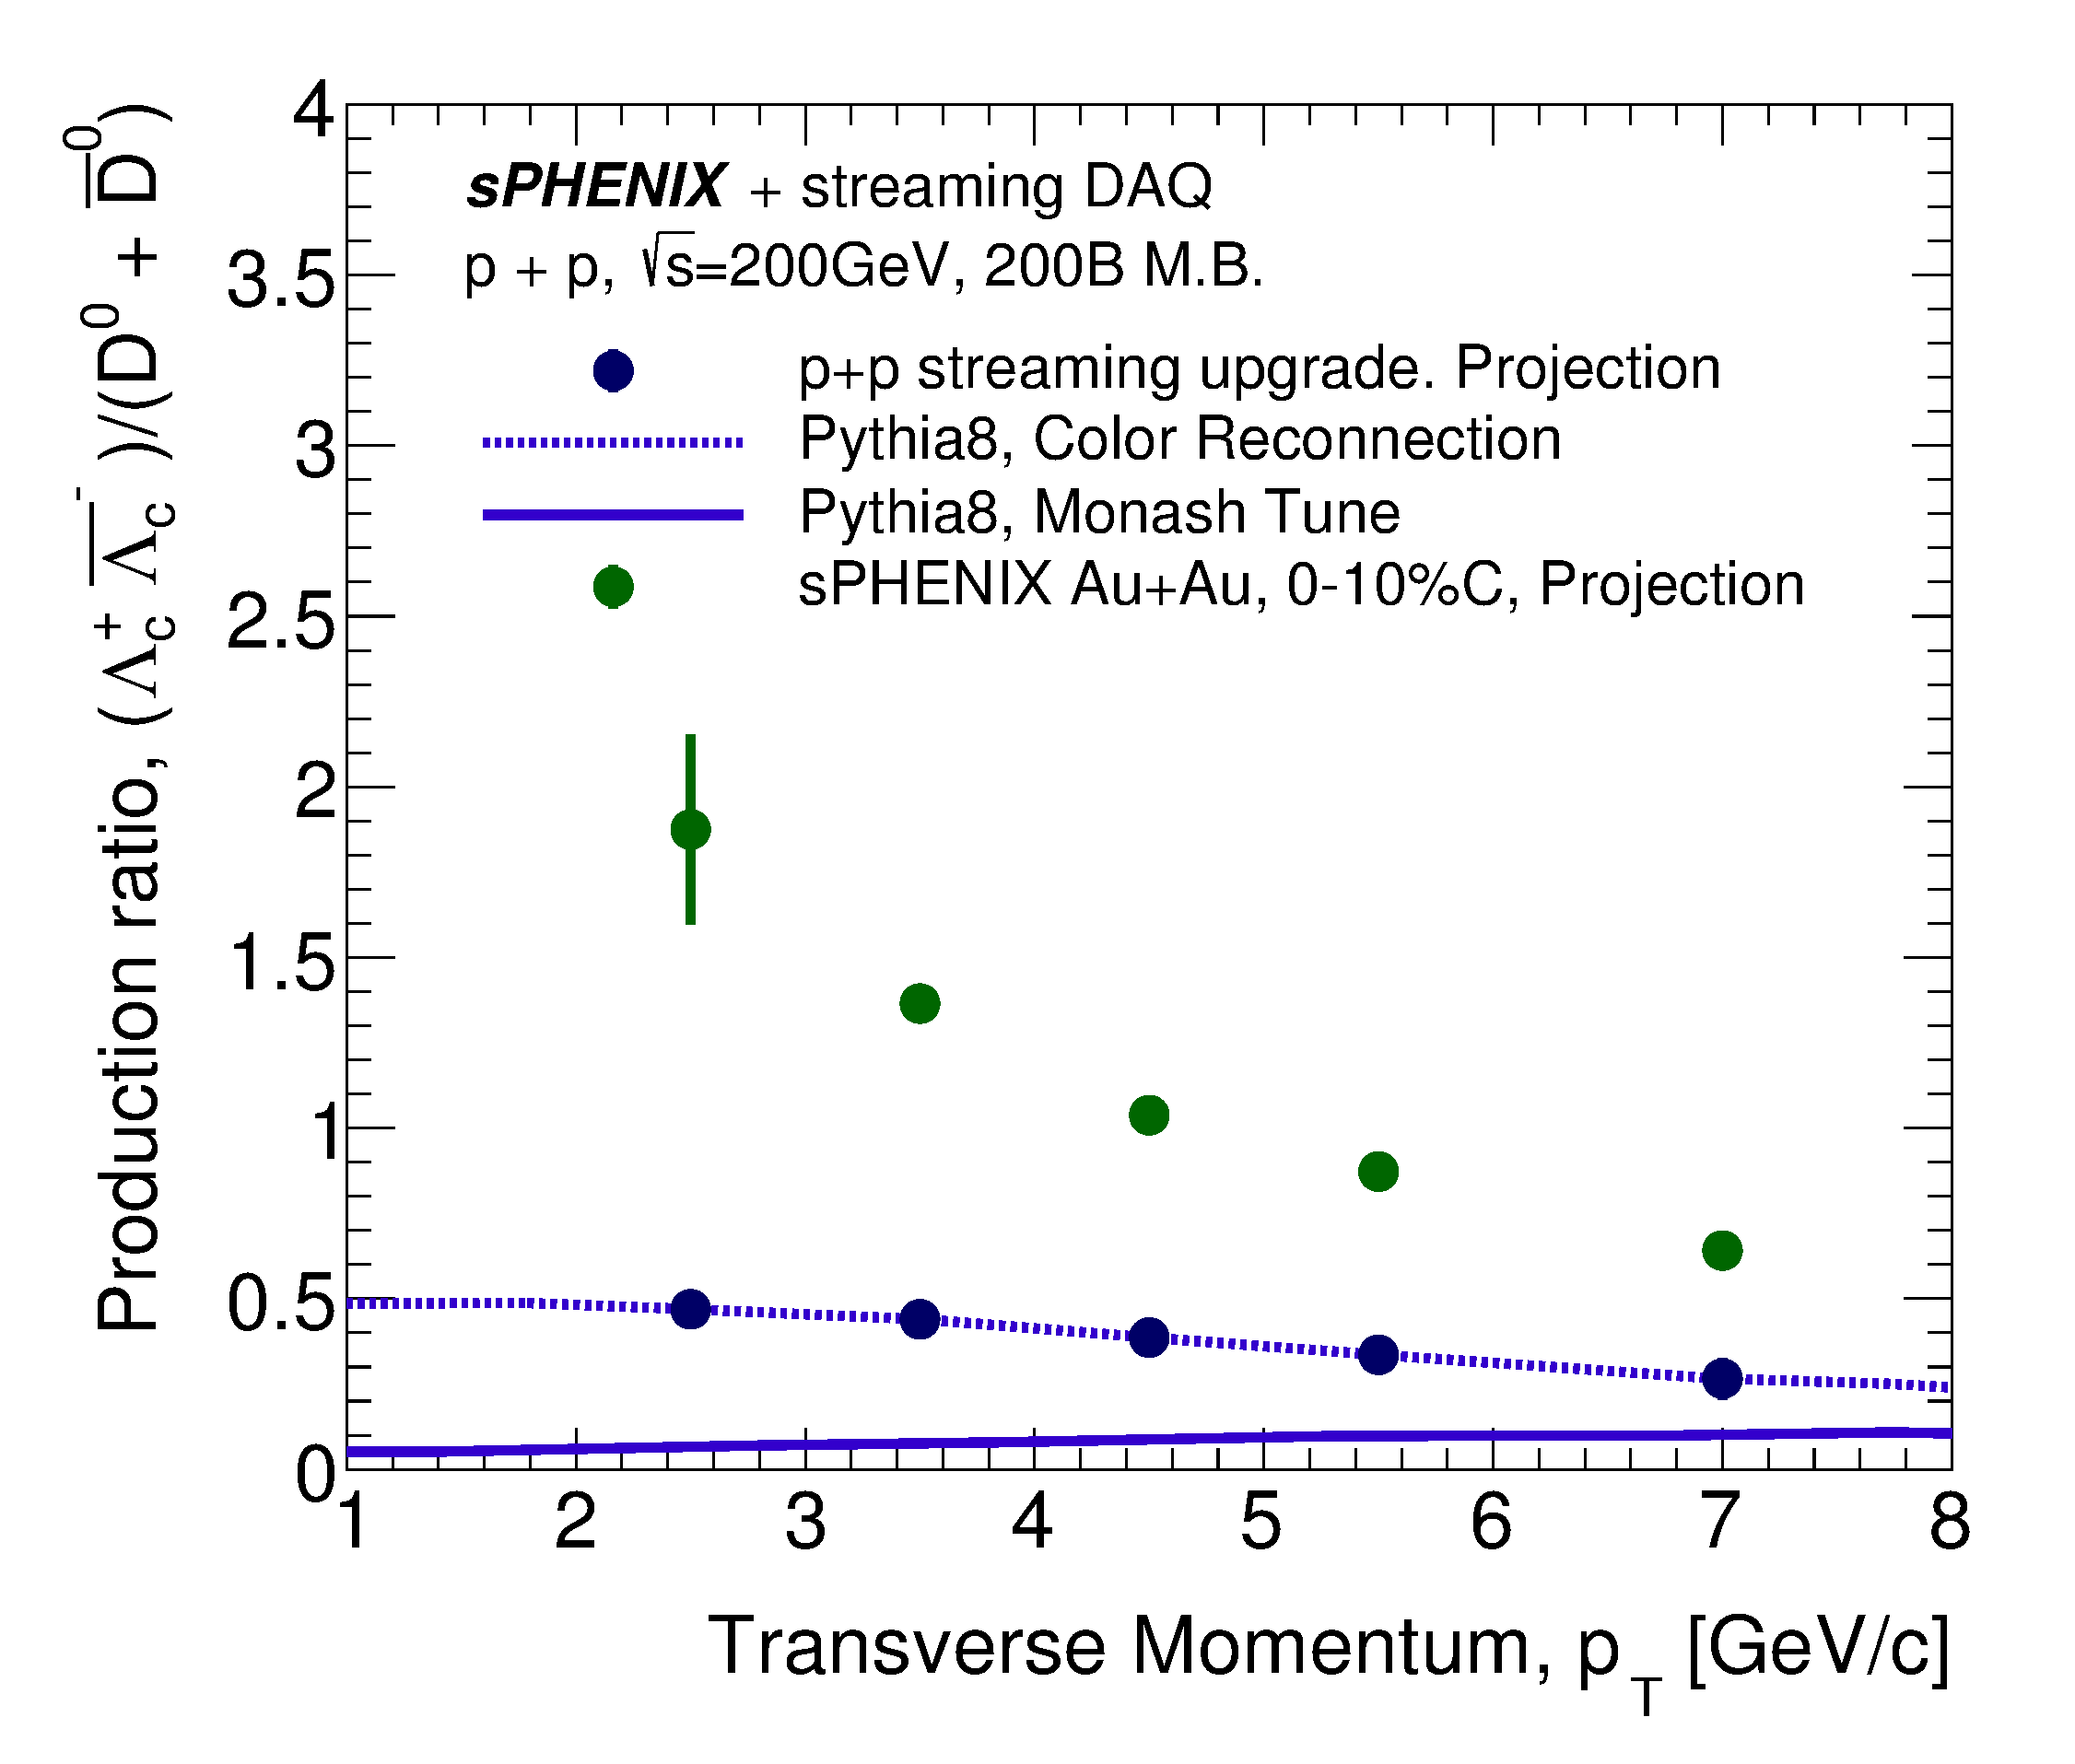
\includegraphics[width=.49\linewidth]{figs/RAA_DB_theory_root_LcD0Ratio_pp200B.pdf}
% 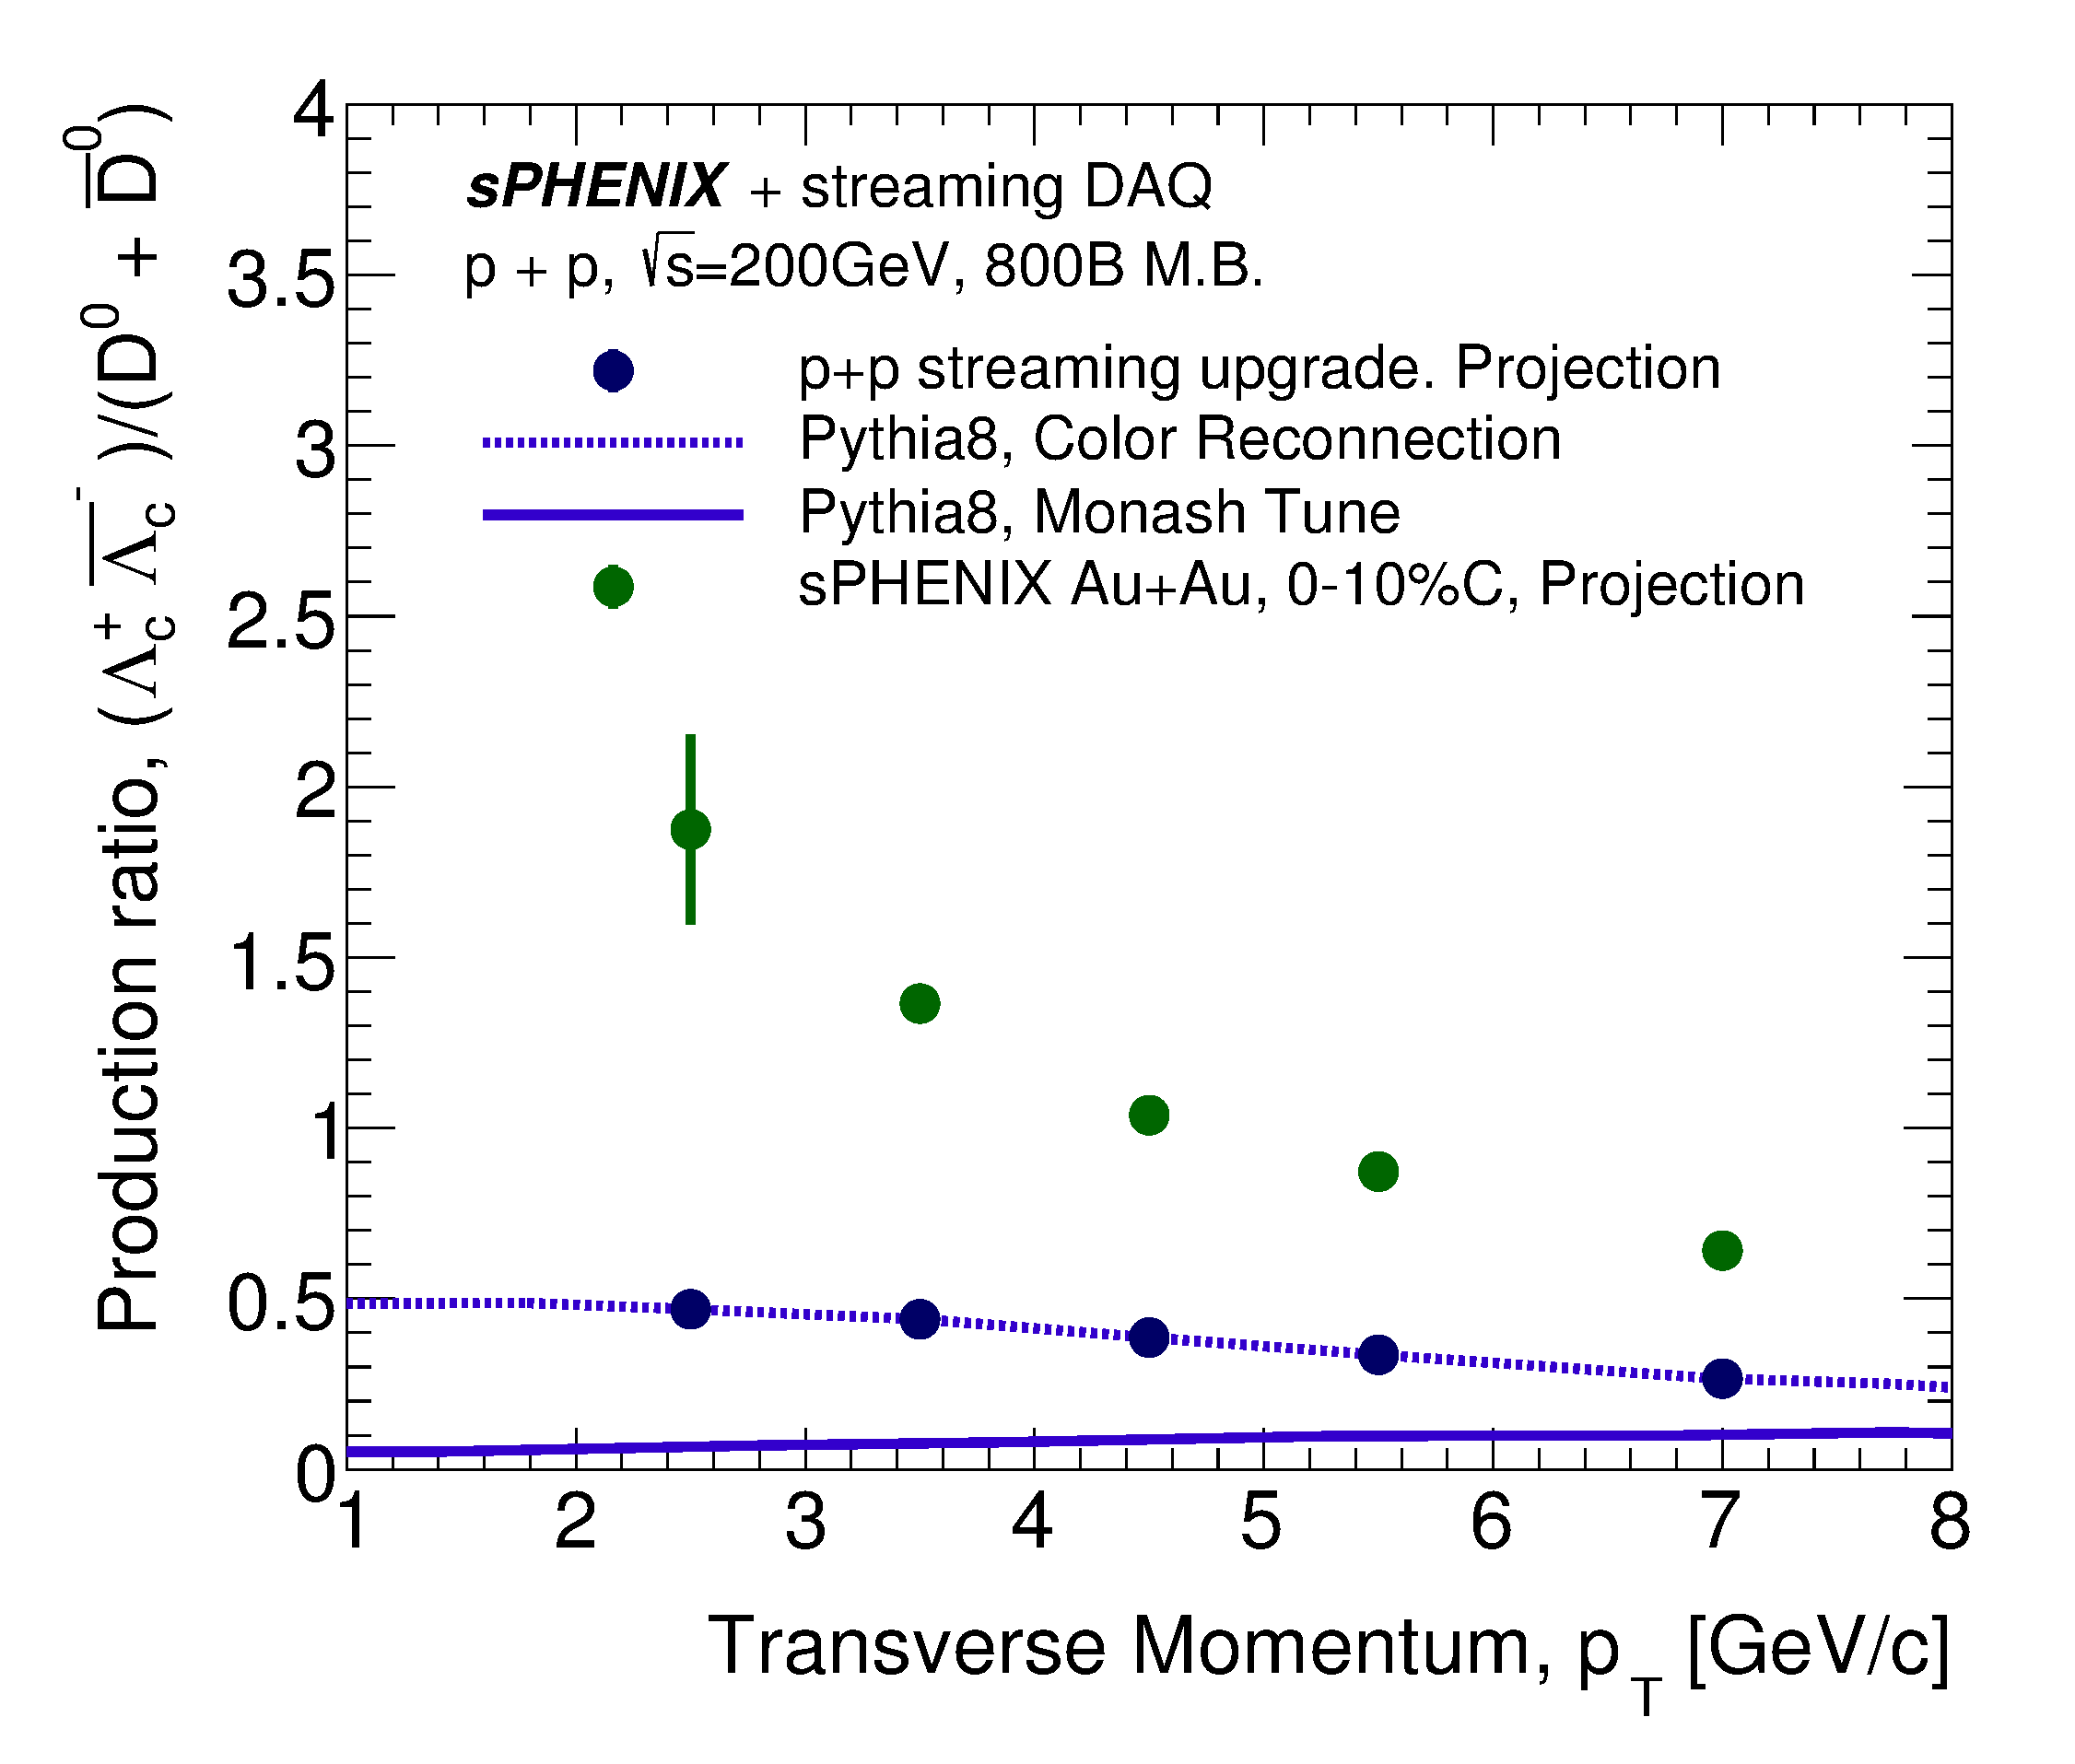
\includegraphics[width=.49\linewidth]{figs/RAA_DB_theory_root_LcD0Ratio.pdf}
\caption{Statistical projections of $\Lambda_c/D$ ratio for Year-2 data taking.}
\label{fig:Lc-D0}
\end{center}
\end{figure}



Recent RHIC and LHC data indicate significant enhancements of the  $\lambda_c$ baryon to $D^0$ meson production ratio in \pp,  \pA and \aa  collisions []. However, the reference $\Lambda_c/D$ ratio in the \pp collision is missing at the RHIC energies, and the current model predictions differ significantly. As shown in Figure~\ref{fig:Lc-D0}, this upgrade will enable the first measurement of the $\Lambda_c/D$ in \pp collisions at RHIC and provide the critically missing link to quantitatively understand the enhancement of the charmed baryon/meson production ratio and therefore charm hadronization in the QGP []. 


\section{Gluon Dynamics and Single Spin Asymmetry}



\begin{figure}[htbp]
\begin{center}
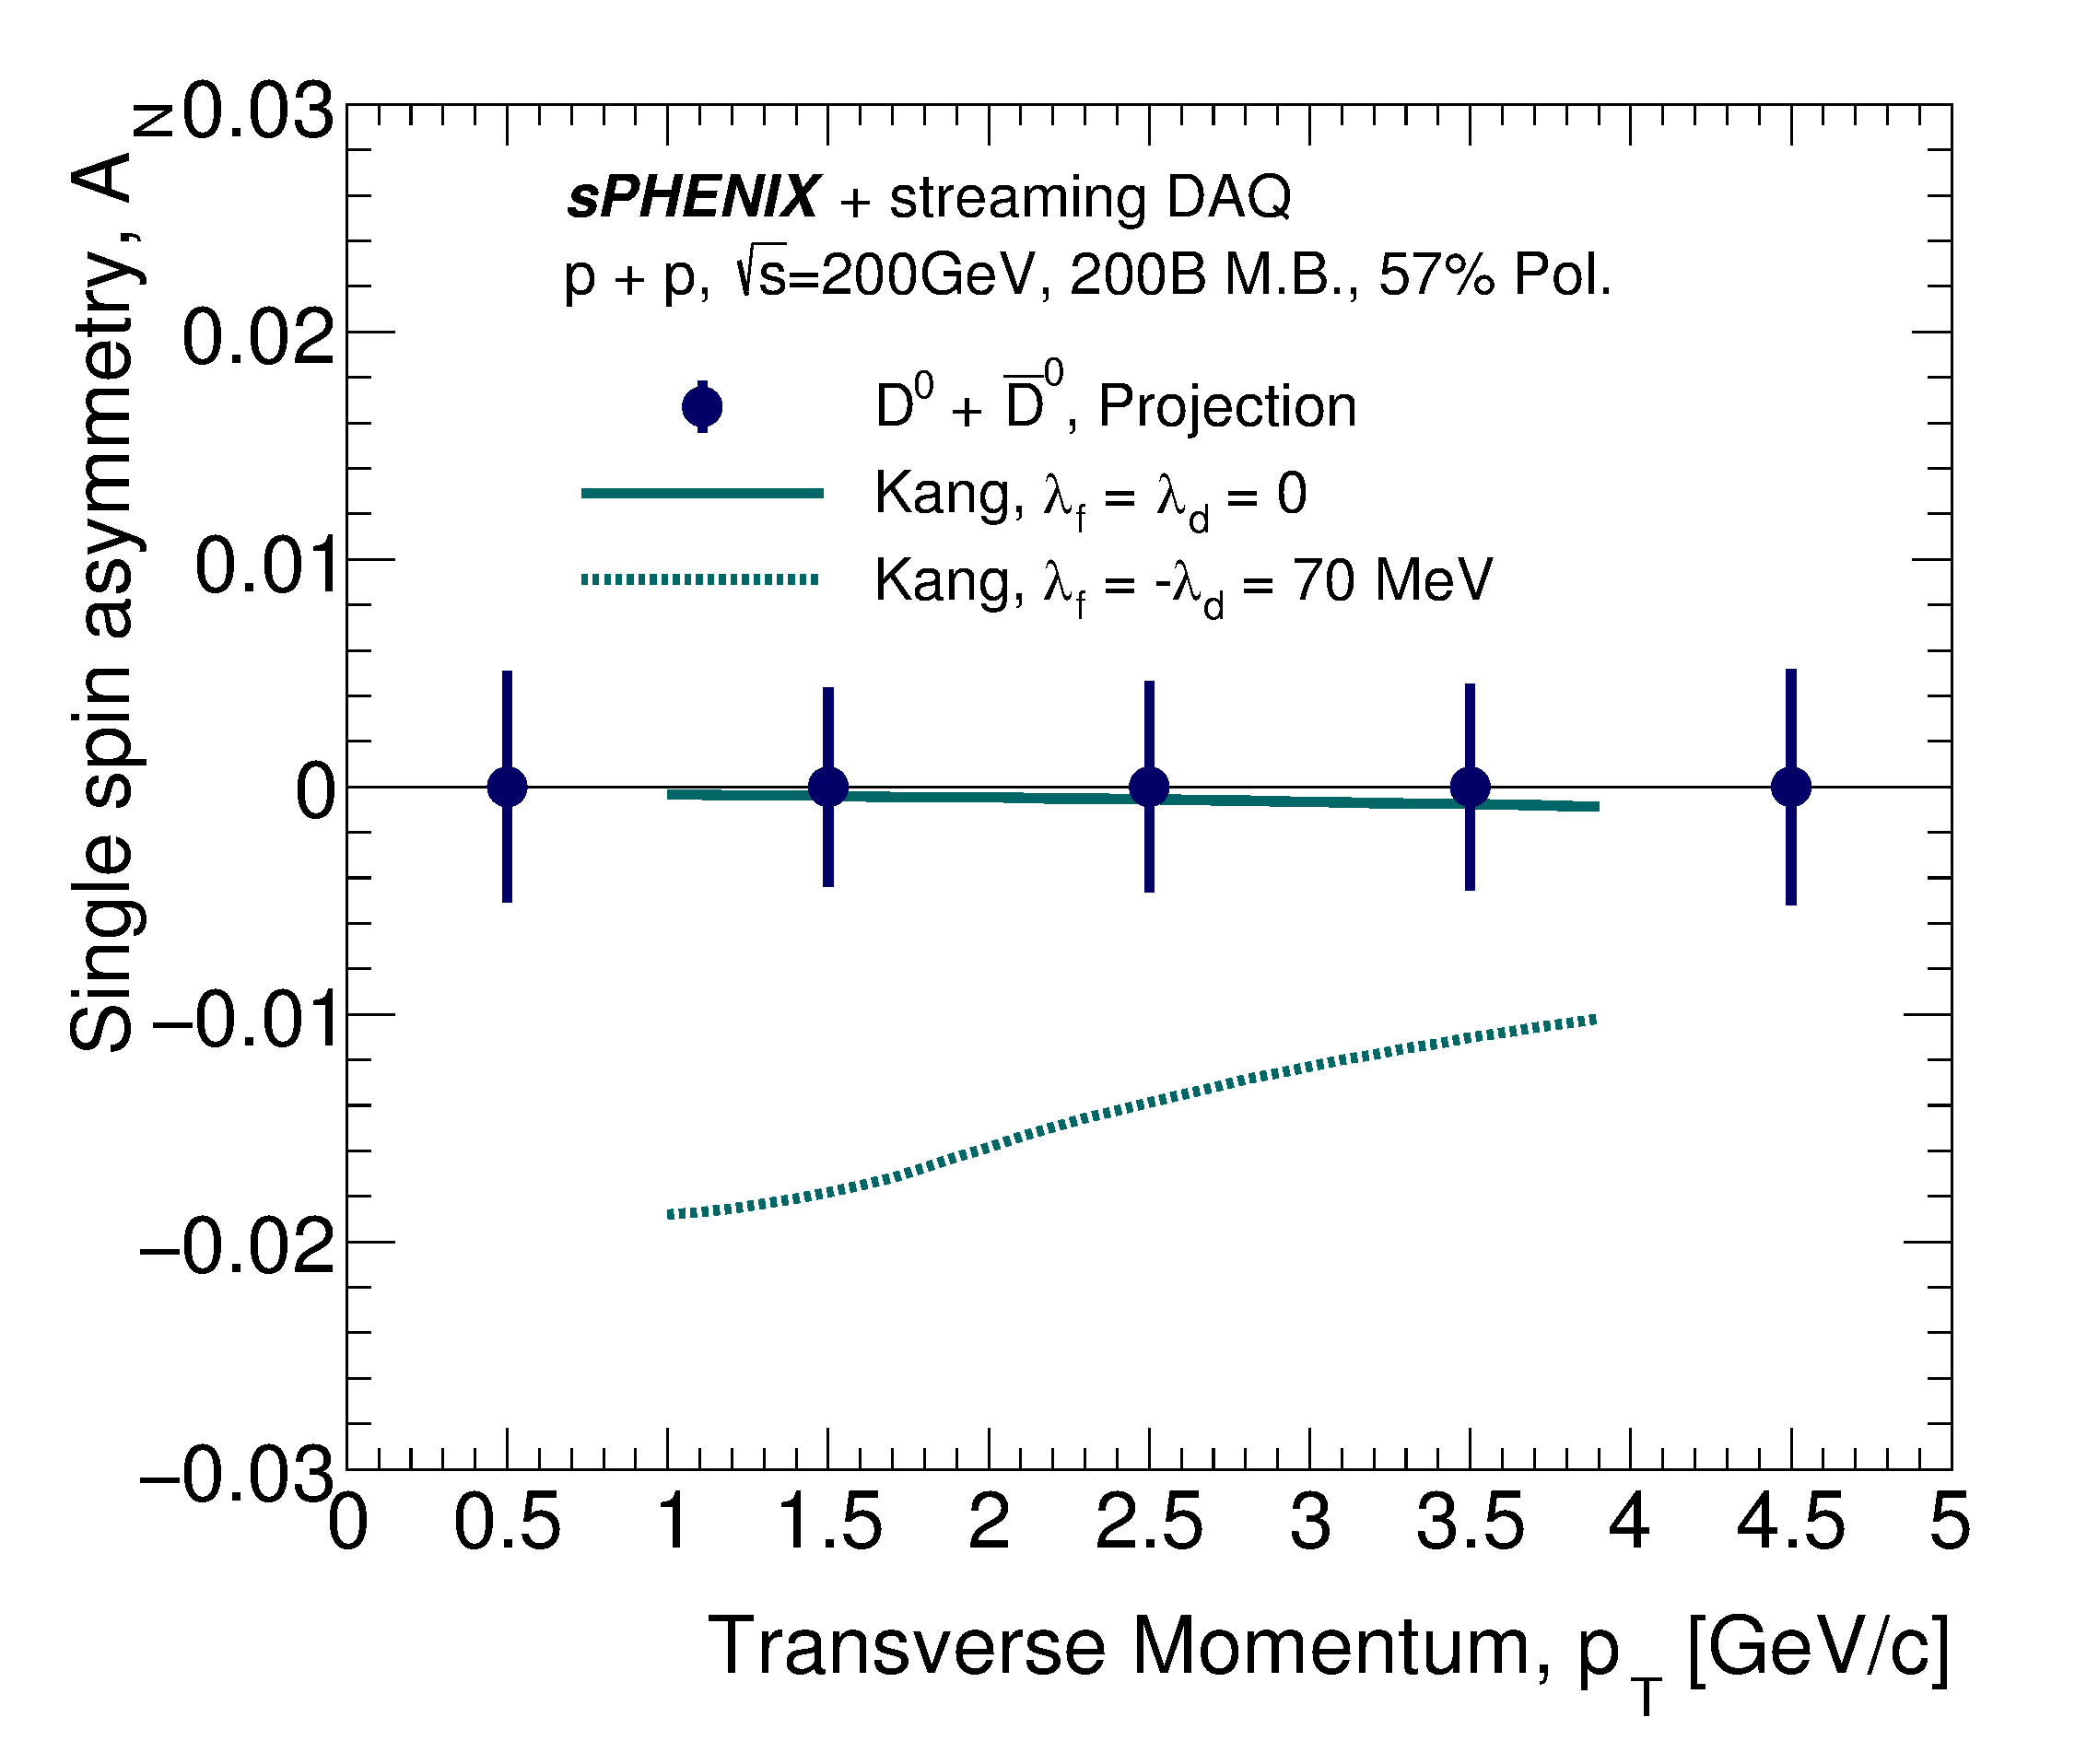
\includegraphics[width=.49\linewidth]{figs/RAA_DB_theory_root_AN_D0D0bar_pp200B.pdf}
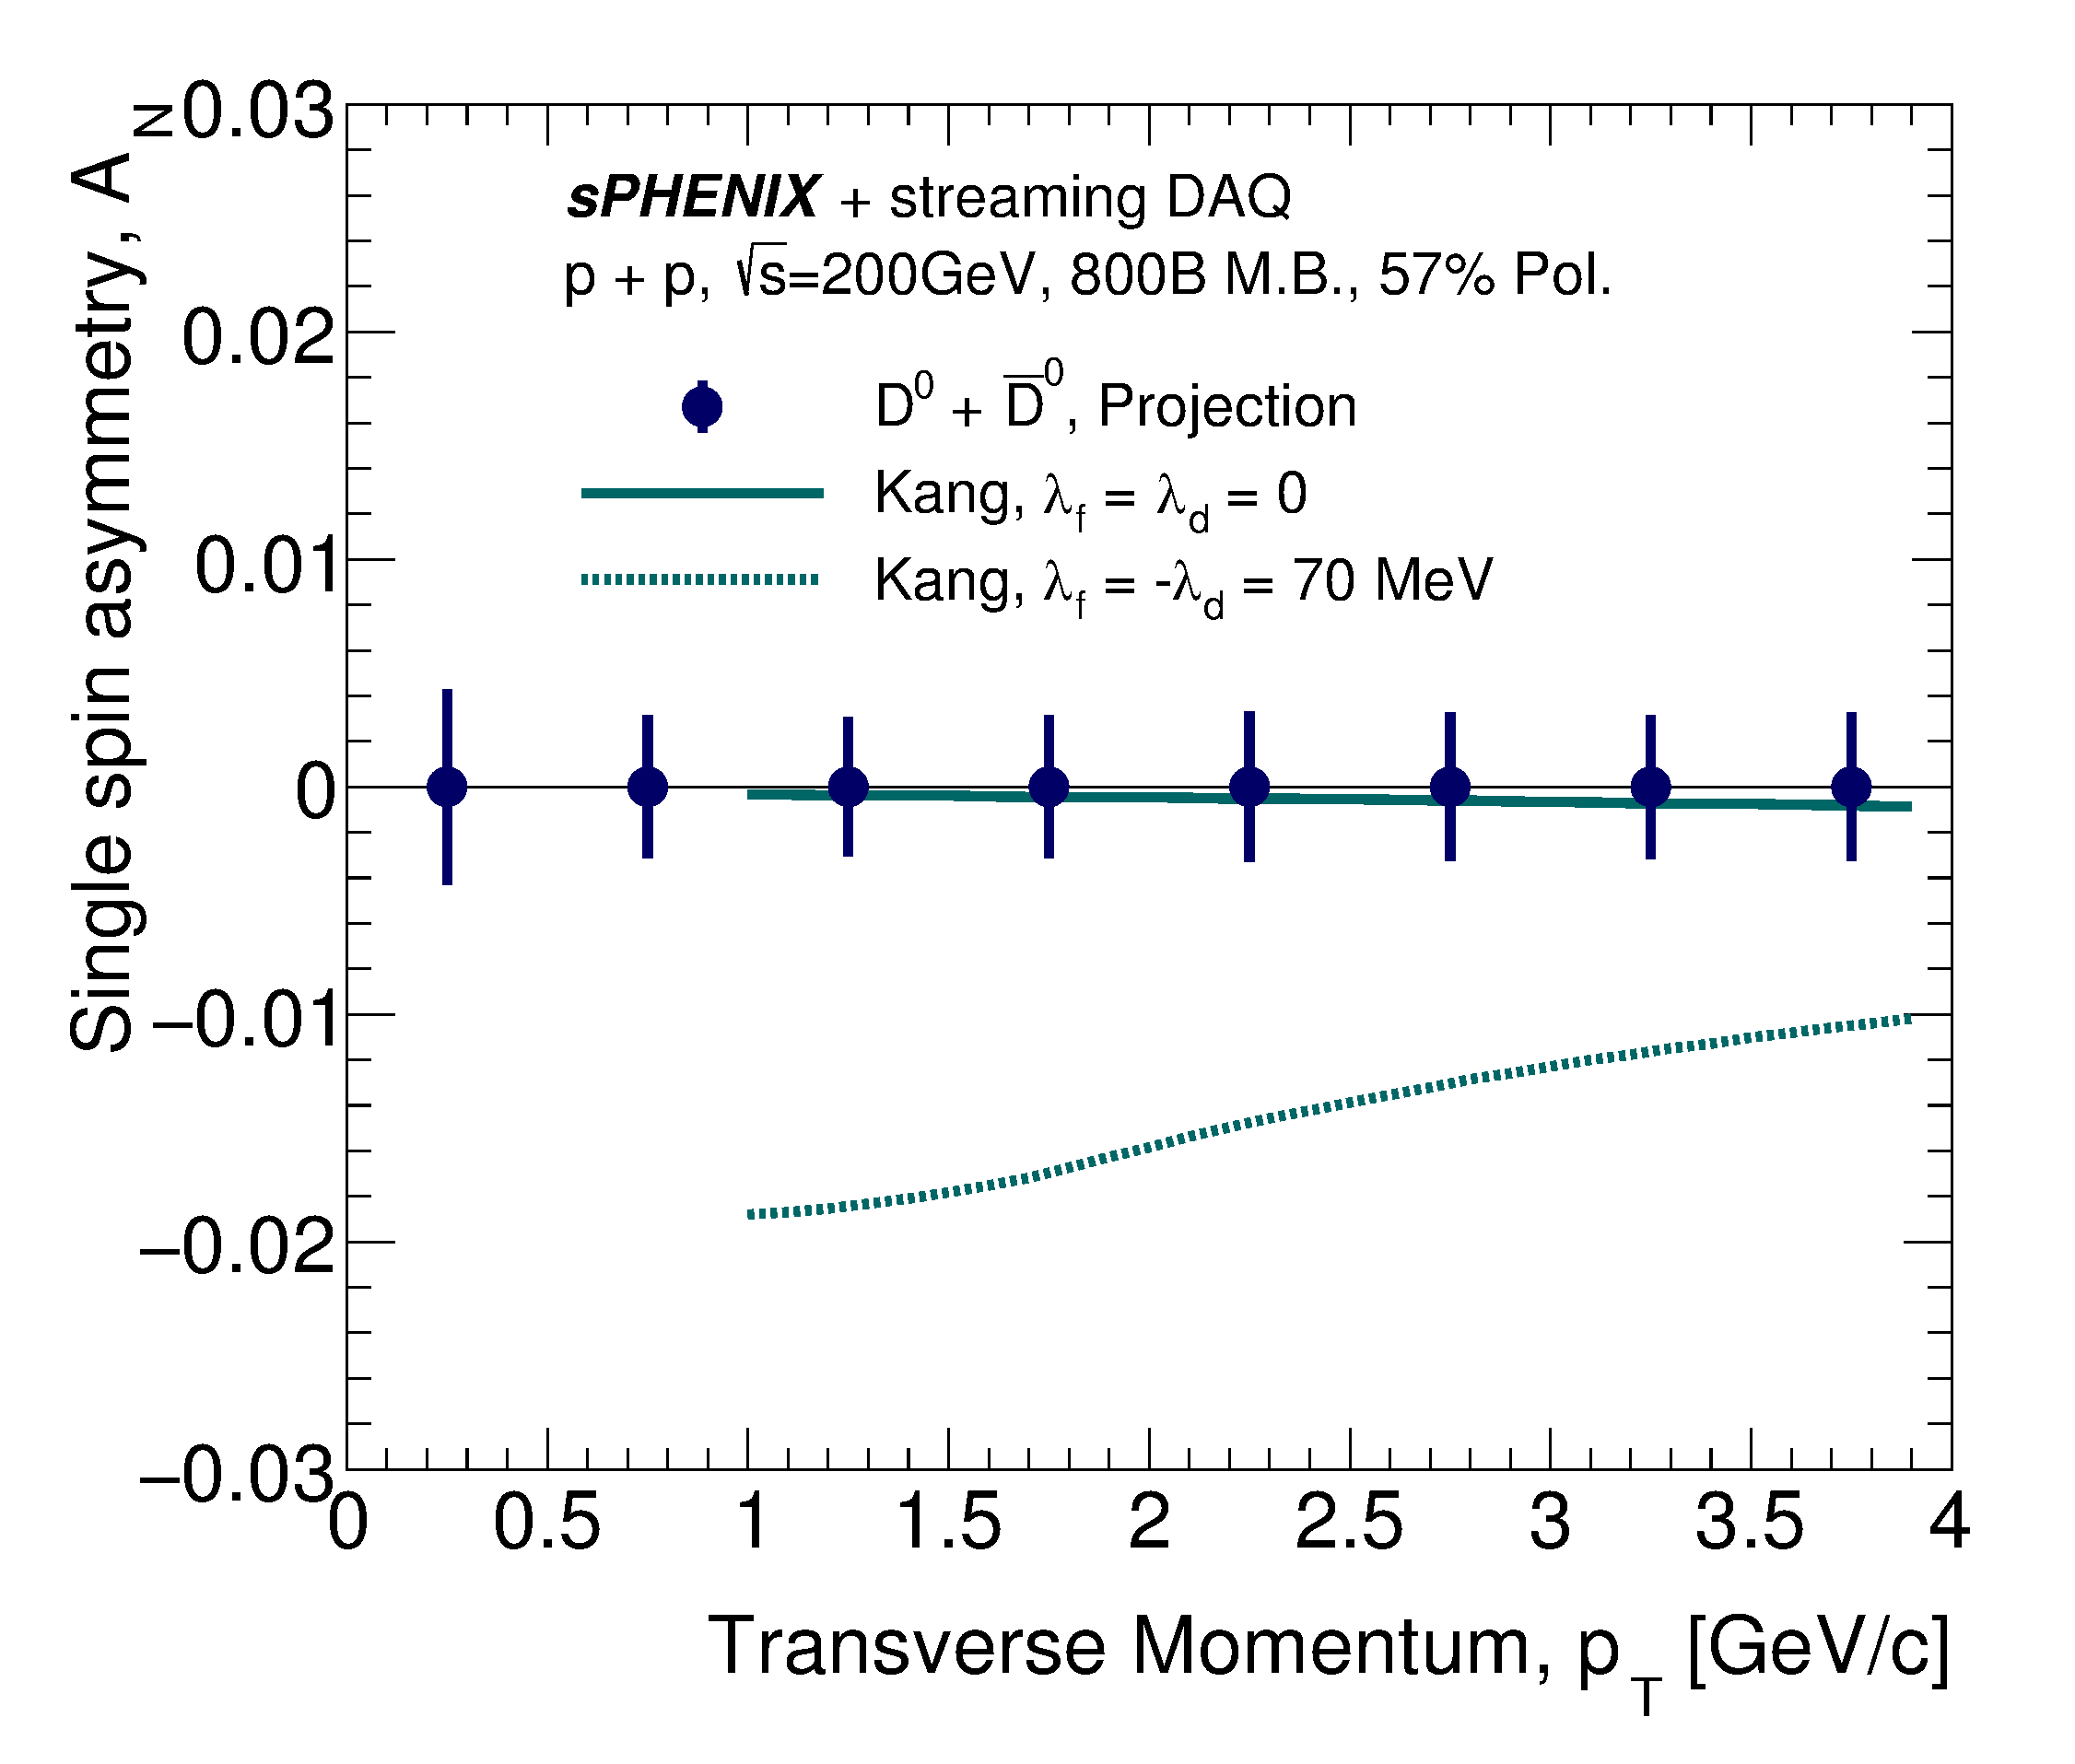
\includegraphics[width=.49\linewidth]{figs/RAA_DB_theory_root_AN_D0D0bar.pdf}
\caption{Statistical projections of transverse spin asmmetry for the $D^0$ mesons for Year-2 and Year 2+4 data taking.}
\label{fig:AN-D0}
\end{center}
\end{figure}


RHIC is a unique collider that is capable of colliding polarized protons. With transversely polarized proton beams, this dataset will enable a high precision measurement of $D^0$ transverse single spin asymmetry (TSSA) in the mid-rapidity region as shown in Figure~\ref{fig:AN-D0}. This observable is a unique probe of the twist-3 tri-gluon correlation function and gluon Sievers effect in the polarized proton, which opens a new window into the dynamics of gluons in hadrons [?]. 
 

\section{Bridging the gap in nuclear dependent $A_N$ mystery}

- Sasha?
 
 
\section{Data Mining}

This upgrade will accumulate a large amount (200 billion) of minimal bias polarized \pp collision without a triggering-bias and with the full sPHENIX tracking capability. After RHIC completes its scientific mission at the end of the sPHENIX program, this would be a unique dataset allowing future data mining for novel quantum effects such as the quantum coherence in particle productions. These \pp data may be critical in understanding the future $e+p/A$ collision data at an EIC [?]. 